\section{Direkte Anrufe} \label{sec:privatecall}
Direktrufe (\aref{Private Call}) ermöglichen es mit einem anderen Teilnehmer direkt zu kommunizieren, ohne dabei weitere Teilnehmer zu stören (bis auf das Belegen eines Repeaters). Im Rahmen der DMR Einführung wurde der Direktruf auch über mehrere Repeater hinweg beschrieben. Eben dieser Aspekt von DMR ist meiner Meinung nach besonders interessant. Mit Ausnahme der Sprechgruppen 8 \& 9 (siehe Abs. \ref{sec:lokal}), sind Direkt- und Gruppenrufe in DMR transparent gegenüber den verwendeten Repeatern. Es spielt keine Rolle über welchen Repeater sich Teilnehmer an einem Direktruf beteiligen und somit auch nicht wo sie sich befinden. 

\begin{figure}[!ht]
 \centering
 \documentclass{standalone}
\usepackage{tikz}
\usetikzlibrary{shapes.geometric}
\newcommand{\repeater}[3]{%
 \node ({#1}) at ({#2}) {%
  \begin{tikzpicture}%
   \draw [black,thick] (-.25,0) -- (0,0.5) -- (0.25,0) -- (-0.25,0);%
   \draw [black,thick,domain=-45:225] plot ({0.2*cos(\x)}, {0.5+0.2*sin(\x)});%
   \draw [black,thick,domain=-45:225] plot ({0.4*cos(\x)}, {0.5+0.4*sin(\x)});%
   \node (xxx) at (0,-.2) {{#3}};%
  \end{tikzpicture}%
 } %
}

\newcommand{\activerepeater}[3]{%
 \node ({#1}) at ({#2}) {%
  \begin{tikzpicture}%
   \draw [black,thick] (-.25,0) -- (0,0.5) -- (0.25,0) -- (-0.25,0);%
   \draw [red,thick,domain=-45:225] plot ({0.2*cos(\x)}, {0.5+0.2*sin(\x)});%
   \draw [red,thick,domain=-45:225] plot ({0.4*cos(\x)}, {0.5+0.4*sin(\x)});%
   \node (xxx) at (0,-.2) {{#3}};%
  \end{tikzpicture}%
 } %
}


\newcommand{\user}[3]{%
 \node ({#1}) at ({#2}) {%
  \begin{tikzpicture}%
   \draw [black,fill=black] (-.25,0) -- (0,0.5) -- (0.25,0) -- (-0.25,0);%
   \draw [black,fill=black] (0,.5) circle (.2); %
   \node (xxx) [text width=0.6cm, align=center] at (-.35cm,-.4) {{#3}};%
  \end{tikzpicture}%
 } %
}

\newcommand{\activeuser}[3]{%
 \node ({#1}) at ({#2}) {%
  \begin{tikzpicture}%
   \draw [red,fill=red] (-.25,0) -- (0,0.5) -- (0.25,0) -- (-0.25,0);%
   \draw [red,fill=red] (0,.5) circle (.2); %
   \node (xxx) [text width=0.6cm, align=center] at (-.35cm,-.4) {{#3}};%
  \end{tikzpicture}%
 } %
}

\begin{document}
 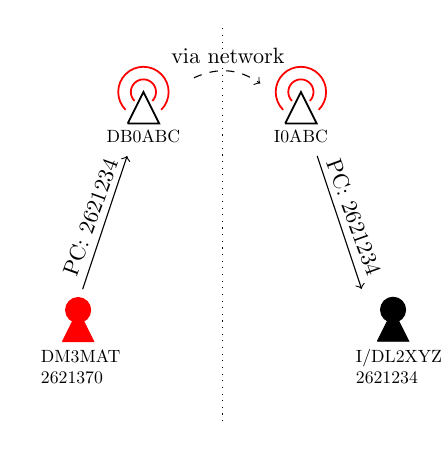
\begin{tikzpicture}[every node/.style={scale=.8}]
  \activeuser{u1}{ 0,0}{DM3MAT 2621370};
  \activerepeater{R1}{1,3}{DB0ABC};
  \draw[dotted] (2,4) -- (2,-1);
  \user{u2}{ 4,0}{I/DL2XYZ\\2621234};	
  \activerepeater{R2}{3,3}{I0ABC};
  \draw[->] (u1) -- node[above,rotate=70]{PC: 2621234} (R1);
  \draw[->] (R2) -- node[above,rotate=-70]{PC: 2621234} (u2);
  \path[->] (R1) edge[dashed,bend left] node[above]{via network} (R2);
 \end{tikzpicture}
\end{document}

 \caption{Beispiel eines Direktrufs über Ländergrenzen hinweg.} \label{fig:pc}
\end{figure}

Das heißt, YLs \& OMs\footnote{Für nicht-Funkamateure: Zwei weitere typische Abkürzungen im Amateurfunk die \emph{young lady} und \emph{old man} bedeuten und alle weiblichen b.z.w. männlichen Funkamateure bezeichnet.}, die sich im Urlaub aufhalten, können wie gewohnt an ihren lokalen Nachmittagsrunden teilnehmen, indem sie am Urlaubsort einen DMR Repeater auswählen und von dort aus einen Gruppenruf zu ihrer Sprechgruppe in der Heimat starten. Damit abonnieren sie ihre Sprechgruppe an ihrem Urlaubsrepeater temporär und dieser verhält sich danach wie ein Repeater der in der Heimat steht. 

Ebenso können sie Direktrufe vom Urlaubsort an Bekannte absetzen und am Urlaubsort empfangen. Vorausgesetzt, sie haben sich durch kurzes drücken auf die PTT Taste beim Repeater am Urlaubsort angemeldet, damit das DMR Netz weiß, wo der Teilnehmer zu finden ist. Damit müssen die Teilnehmer in der Heimat aber nicht mehr wissen wie und wo sie den Urlauber erreichen können. Sie starten einfach einen Direktruf zum Urlauber und das DMR Netz kümmert sich um alles.

In Abbildung \ref{fig:pc} ist eben solch ein Direktruf über Ländergrenzen hinweg dargestellt. DM3MAT ruft via seinem lokalen Repeater (DB0ABC) den Urlauber DL2XYZ per Direktruf an. Da sich dieser bei einem DMR Repeater (I0ABC) an seinem Urlaubsort in Italien angemeldet hat\footnote{Um sich an einem Repeater anzumelden, damit das Netzwerk weiß, dass man über diesen Repeater erreichbar ist, drückt man kurz die PTT Taste auf einem Kanal des Repeaters.}, kann der Direktruf an DL2XYZ vermittelt werden. Um diesen Direktruf durchzuführen, muss DM3MAT nicht wissen über welchen Repeater der Urlauber DL2XYZ erreichbar ist. Diese Eigenschaft des DMR Netzes stellt eine deutliche Vereinfachung gegenüber dem \aref{Echolink} Netzwerk dar. 